\documentclass[11pt]{article}

\usepackage[utf8]{inputenc}
\usepackage{amsfonts,amsmath,amssymb,amsthm} % math
\DeclareMathOperator{\tr}{tr} % \tr operator
\DeclareMathOperator{\sgn}{sgn} % \sgn operator
\DeclareMathOperator*{\argmax}{arg\,max\,} % \argmax operator
\usepackage[german, english]{babel} % language
\usepackage[margin=2cm]{geometry} % page margins
\usepackage{graphicx} % images
\usepackage{caption} % dependency of subcaption
\usepackage{subcaption} % subfigures

\renewcommand{\labelitemi}{$\bullet$}
\renewcommand{\labelitemii}{$\diamond$}
\renewcommand{\labelitemiii}{$\vartriangleright$}
\renewcommand{\labelitemiv}{\textbf{-}}

\title{\textbf{Bildverstehen II}}
\date{\today}

\author{
  Benkel, Sebastian
  \and
  Bernecker, Tobias
  \and
  Wudenka, Martin
}

\begin{document}

\maketitle

\section{Merkmalsextraktion}

\subsection{Maßstabsraum-Repräsentation von Bildern}
% Wichtige Punkte, die man sich merken sollte
%  Definition und Extraktion von Linienpunkten und Linienbreite
%  Glättung führt inhärent zu verzerrten Extraktionsergebnissen
%  Durch geeignete Modellierung können die Verzerrungen korrigiert
% werden
%  Prinzip der maßstabsraumbasierten Linien- und Kantenextraktion
%  Prinzip des Strukturtensors
%  Ansatz des Harris-Punktextraktors
%  Ansatz des Förstner-Punktextraktors
%  Ansatz des Lepetit-Punktextraktors
\begin{itemize}
    \item Maßstab: n-Meter/Pixel
        \begin{itemize}
            \item Kleinmaßstäblich(über den Bruch definiert): Objekte werden kleiner dargestellt
            \item Großmaßstäblich: Objekte werden größer dargestellt
            \item Auch Maß dafür wieviel Information über Details in einer Karte vorhanden sind
            \item Auflösung: Fähigkeit feine Strukturen zu unterscheiden(dichte Punkte als solche erkennen)
            \item Glättung reduziert Auflösung
            \item Glättungsfilter $L(f,t)$: $f(p)$ = Bild, $t$ = Maßstab(scale, quasi Kernelsize)
        \end{itemize}
    \item Maßstabsraum-Axiome, Gaußfilter
    \begin{itemize}
        \item Linearität (das Bild ist eine Überlagerung von Signalen)
        \item Positionsinvarianz (der betrachtete Ausschnitt der Welt ist irrelevant)
        \item Rotationsinvarianz (die Orientierung, in der die Welt betrachtet wird, ist irrelevant)
        \item Halbgruppeneigenschaft (Reduktionen der Auflösung kombinieren sich linear)
        \item Vernichtung von Maxima mit größeren t : Formalisierung der Reduktion der Auflösung
        \item Der Gauß-Filter ist der einzige Filter, der alle Maßstabsraum-Axiome erfüllt
        \item Gauß: Maßstab t ist gegeben durch $\sigma = t^2$, Merkregel: Objekte, die kleiner als ungefähr $\sqrt{t}$ sind, werden unterdrückt
        \item Diskretes Analogon des Gauß-Filter: Kernel mit entsprechenden (abgetasteten) Werten
    \end{itemize}
\end{itemize}

\subsection{Unterschiedliche Typen von Linienprofilen für unterschiedliche Anwendungen}
\begin{itemize}
    \item Balkenförmiges Linienprofil
    \begin{itemize}
        \item Bei (näherungsweise) parallele Kanten
        \item Bei homogenen Grauwerte innerhalb des Objekts
    \end{itemize}
    \item Parabolisches Linienprofil
    \begin{itemize}
        \item Röhrenförmige Objekte die im Durchlicht aufgenommen werden (Objekte werden scharf abgebildet (optisch, Röntgen))
    \end{itemize}
    \item Gaußsches Linienprofil
    \begin{itemize}
        \item Röhrenförmige Objekte die im Durchlicht aufgenommen werden (Objekte werden unscharf abgebildet, liegen in streuendem Medium, (optisch, Röntgen))
    \end{itemize}

\end{itemize}
\subsection{Definition und Extraktion von Linienpunkten und Linienbreite}
    Merkmalsextraktion:
        \begin{itemize}
            \item Kanten
            \begin{itemize}
                \item Zu extrahierende Merkmale werden häufig über Differentialinvarianten beschrieben und extrahiert
                \item Kante $\Leftrightarrow$ Maximum des Gradientenbetrags in Richtung des Gradienten $\Leftrightarrow$ Nullstelle der zweiten Richtungsableitung in Richtung des Gradienten
                \item lokales orthonormales Koordinatensystem $(u, v)$, $v$ parallel - $u$ senkrecht zum Gradienten
            \end{itemize}
        \item Linien
            \begin{itemize}
                \item Besitzen charakteristisches Grauwertprofil senkrecht zum Linienverlauf
                \item Balkenförmiges Linienprofil (Straßen, parallele Kanten und homogene Grauwerte innerhalb des Objekts)
                \item Parabolisches Linienprofil (Blutgefäße im Röntgenbild, röhrenförmige Objekte im Durchlicht (scharf))
                \item Gaußsches Linienprofil (Blutgefäß im optischen Bild, röhrenförmige Objekte im Durchlicht (unscharf))
                \item Asymetrisches Linienprofil: Bsp. Balken:
                    $$f_b(x) = \begin{cases}
                        0, & x < -w \\
                        1, & \|x\| \le w \\
                        a, & x > w
                    \end{cases}$$
                \item $w =$ Linienbreite (halber Durchmesser der Linie), $[0, 1] \ni a =$ Differenz Intensität rechte Seite, linke Seite
                \item Linienbreiten der drei Modelle auf einer Linie sind nicht vergleichbar, ggf. durch gleiche „Gesamtenergie“ oder auf Bruchteil c des Ziel-Grauwerts
                \item für parabolische/Gaußsche Linien gilt: Die Position der Linie ist am lokalen Maxima bzw. Minima des Liniendurchschnitts
                \item Bild muss geglättet werden um balkenförmige Linien zu erkennen, bei den anderen zur Rauschunterdrückung
                \item sichere Linienselektion für Balkenförmige Linine nur möglich bei $\sigma \geq w / \sqrt{3}$ für Parabol- und Gaußlinien, $\sigma \geq 0$
                \item zur Steigerung der Performance wird $\sigma$ konstant gehalten und w variiert
                \item Linienbreite und Mittel
            \end{itemize}
        \end{itemize}
    Extraktion der Linienposition:
    \begin{itemize}
        \item Vektor horizontal zur Linie ist duch Eigenvektor zum betragsmäßig größeren Eigenwert der
            Hessematrix gegeben. Dieser und Maximum bzw. Minimum der Richtungsableitung geben Linienmittelpunkt und Ausrichtung pro Pixel/Auswertung
    \end{itemize}

\subsection{Glättung führt inhärent zu verzerrten Extraktionsergebnissen}
    Maßstabsinvarianz:
        \begin{itemize}
            \item Linienkanten und Mittelpunkt werden proportional verzerrt
            \end{itemize}

\subsection{Durch geeignete Modellierung können die Verzerrungen korrigiert werden}
            \begin{itemize}
            \item Verzerrung der Breite und der Linienposition kann für ein Bild ermittelt und weitestgehend korrigiert werden
            \item Dank Maßstabsinvarianz (Fehler skaliert) reicht ermitteln der Invarianz für $\sigma = 1$
        \end{itemize}

\subsection{Prinzip der maßstabsraumbasierten Linien- und Kantenextraktion}
\subsection{Prinzip des Strukturtensors}

\begin{itemize}
    \item Viele Punktextraktoren basieren auf dem Strukturtensor
    \item Bild $f$ mit Gradient $\nabla f = (f_r, f_c)$
    \item Strukturtensor $\boldsymbol{S}(r, c) = w(r, c) \ast \big(\nabla f(r, c)^T \nabla f(r, c)\big) = w(r, c) \ast \begin{pmatrix} f_r(r, c)^2 & f_r(r, c) f_c(r, c) \\ f_r(r, c) f_c(r, c) & f_c(r, c)^2 \end{pmatrix}$
    \item Als Gewichtung wird meistens der Gaußfilter verwendet $w(r, c) = \sigma(r, c; \sigma_i)$, wobei $\sigma_i$ als Integrationsmaßstab bezeichnet wird
    \item Im Diskreten Ableitungen des Bildes über finite Differenzen, aber oft Ableitungen des Gaußfilters stattdessen verwenden: $(f_r(r, c), f_c(r, c)) := (g_r(r, c; \sigma_g), g_c(r, c; \sigma_g)) \ast f(r, c)$ ($\sigma_g$: lokaler Maßstab)
    \item Eigenwerte $\lambda_1 \ge \lambda_2 \ge 0$ und Eigenvektoren $e_1, e_2$ des Strukturtensors liefern Informationen über den Inhalt des Integrationsfensters:
        \begin{itemize}
            \item $\lambda_1 \approx 0, \lambda_2 \approx 0 \Rightarrow$ Das Integrationsfenster enthält keine Kanten
            \item $\lambda_1 \gg 0, \lambda_2 \approx 0 \Rightarrow$ Das Integrationsfenster enthält Kanten oder Linien; $e_1$ ist die Richtung senkrecht zur Kante oder Linie
            \item $\lambda_1 \gg 0, \lambda_2 \gg 0 \Rightarrow$ Das Integrationsfenster enthält eine Ecke oder einen flächenhaften Punkt
        \end{itemize}
\end{itemize}

\subsection{Ansatz des Harris-Punktextraktors}

\begin{itemize}
    \item Basiert auf dem Strukturtensor
    \item Zur Unterdrückung von Kanten und zur Vermeidung der teuren Berechnung der Eigenwerte Verwendung der Antwortfunktion $R = \det {(\boldsymbol{S})} - k \tr{ (\boldsymbol{S}) }^2$ mit $R > 0$ und $R$ maximal (pixelgenau)
    \item In der Praxis Verwendung eines höheren Schwellwertes für $R$ und subpixelgenaue Bestimmung der Position der lokalen Maxima 
\end{itemize}

\subsection{Ansatz des Förstner-Punktextraktors}

\begin{figure}[h!]
    \centering
    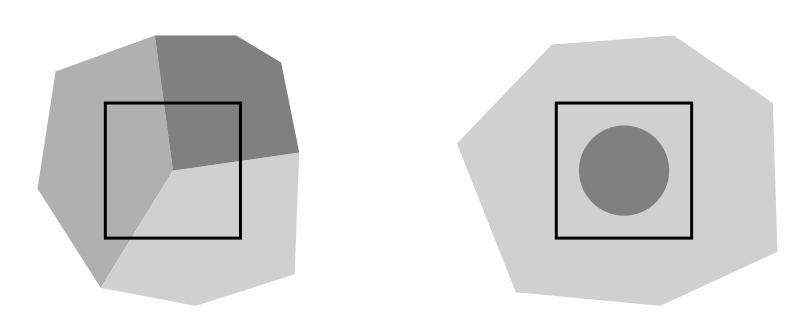
\includegraphics[scale=0.3]{images/punktregionen.png}
    \caption{Kreuzungspunkt und Flächenpunkt.}
    \label{fig:punktregionen}
\end{figure}

\begin{itemize}
    \item Basiert auf dem Strukturtensor
    \item Extrahiert 2D-Merkmale (homogene Regionen), 1D-Merkmale (Kanten, Linien) und 0D-Merkmale (Punkte)
    \item Unterscheidung zwischen homogenen Regionen $H$ und inhomogenen Regionen (Kanten, Linien, Punkte): $(r, c)^T \in H \Leftrightarrow \lambda_1 + \lambda_2 = \tr(\boldsymbol{S}) < t_h$
    \item Unterscheidung zwischen Punkten und Kanten/Linien über das Verhältnis der Eigenwerte des Strukturtensors: $(r, c)^T \in P \Leftrightarrow v = \frac{\lambda_2}{\lambda_1} > t_v$
    \item Aus Geschwindigkeitsgründen Vermeidung der Berechnung der Eigenwerte
    \item Stattdessen Einführung des Formfaktors $q = \frac{4 \det(\boldsymbol{S})}{\tr(\boldsymbol{S})^2} > t_q$
    \item Umrechnung des Schwellwertes $t_v$ in einen Schwellwert für $q$: $t_q = \frac{4 t_v}{(1 + t_v)^2}$
    \item Weitere Klassifikation der Punktregionen in Kreuzungs- und Flächenpunkte (Figure~\ref{fig:punktregionen}):
        \begin{itemize}
            \item In einem idealen Kreuzungspunkt schneiden sich die Kantenrichtungen (Senkrechten der Gradienten) in einem Punkt
            \item In einem idealen Flächenpunkt schneiden sich die Gradientenrichtungen in einem Punkt
        \end{itemize}
\end{itemize}

Berechnung der Punklokalisierungsgüte:
\begin{itemize}
    \item Verschieben eines Fensters über das Bild
    \item Berechnung des Abstandes einer Geraden zum Mittelpunkt des Fensters für jeden Punkt des Fensters unter der Annahme, es liege ein Kreuzungspunkt oder ein Flächenpunkt vor
    \item Summierung der gewichteten Abstände über das Fenster
    \item Gewichtung der Astände über
        \begin{itemize}
            \item Stärke des Gradienten (große Gradienten sind sicherere Kanten und tragen viel Information zur Lokalisierung bei)
            \item Gauß-Funktion mit Mittelwert am Mittelpunk des Fensters und Maßstab $\sigma_p$ (weit vom Mittelpunkt des Fensters entfernte Punkte tragen weniger Information zur Lokalisierung bei)
        \end{itemize}
\end{itemize}

\begin{itemize}
    \item Bestimmung, welcher Punkttyp vorliegt: statistischer Test auf $s_p = D / D^{\perp}$ ($D =$ Punktlokalisierungsgüte)
    \item Klassifikation in:
        \begin{itemize}
            \item Kreuzungspunkt, falls $s_p$ kleiner als eine untere Signifikanzschwelle
            \item Flächenpunkt, falls $s_p$ größer als eine obere Signifikanzschwelle
            \item Undefinierter Punkt
        \end{itemize}
    \item Die Lokalisierung der Punkte erfolgt durch Bestimmung lokaler Minima in $V$ bzw. $V^{\perp}$ ($V = \frac{D}{w}$ und $V^{\perp} = \frac{D^{\perp}}{w}$)
\end{itemize}

\subsection{Ansatz des Lepetit-Punktextraktors}

\begin{figure}[h!]
    \centering
    \begin{subfigure}[c]{0.3\textwidth}
        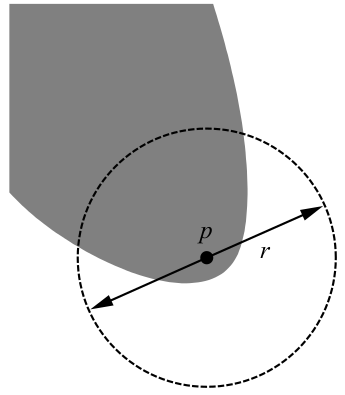
\includegraphics[width=\linewidth]{images/lepetit1.png}
        \subcaption{Lepetit-Ansatz im Kontinuierlichen.}
    \end{subfigure}%
    \begin{subfigure}[c]{0.3\textwidth}
        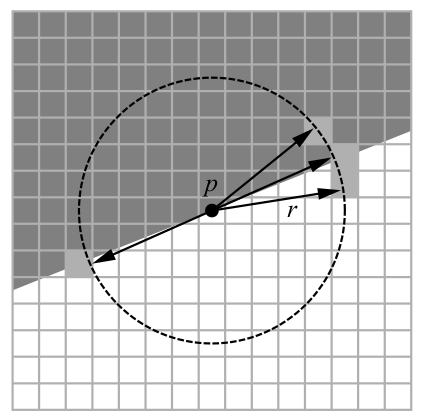
\includegraphics[width=\linewidth]{images/lepetit2.png}
        \subcaption{Lepetit-Ansatz im Diskreten.}
    \end{subfigure}
    \caption{Lepetit-Ansatz.}
    \label{fig:lepetit}
\end{figure}

\begin{itemize}
    \item Harris- und Förstner-Punktextraktoren sind vergleichsweise aufwendig
    \item Geringere Genauigkeit als bei Harris- und Förstner-Punktextraktoren
    \item Für laufzeitkritische Anwendungen (z.B. Objekterkennung)
    \item Liefert stabile markante Punkte
    \item Ansatz (Figure~\ref{fig:lepetit}): Betrachtung der Grauwerte auf einem Kreis um jeden Punkt im Bild \\ $\Rightarrow$ Falls zwei gegenüberliegende Punkte auf dem Kreis ähnliche Grauwerte haben wie der Mittelpunkt, ist der Punkt sicher \underline{kein} markanter Punkt \\ $\Rightarrow$ Falls $\vert f(\boldsymbol{p}) - f(\boldsymbol{p} + \boldsymbol{d}) \vert \leq t_d$ und $\vert f(\boldsymbol{p}) - f(\boldsymbol{p} - \boldsymbol{d}) \vert \leq t_d$ ist $\boldsymbol{p}$ \underline{kein} markanter Punkt ($\boldsymbol{d} = (r \cos \theta, r \sin \theta)^T, \theta \in [0, \pi)$)
    \item Im Diskreten müssen zur Unterdrücken von Antworten an Kanten nicht nur gegenüberliegende Pixel getestet werden, sondern auch noch benachbarte Pixel
    \item Die Tests, ob ein Pixel ein potentieller markanter Punkt ist, sind sehr effizient und können nach dem ersten fehlgeschlagenen Test abgebrochen werden
    \item Nur bei tatsächlichen Kandidaten für markante Punkte wird der gesamte Kreis evaluiert
    \item Die Tests beim Lepetit-Punktextraktor liefern für jeden markanten Punkt mehrere benachbarte Punkte, die die Tests erfüllen
    \item Zur eindeutigen Lokalisierung werden die lokalen Maxima der folgenden Antwortfunktion berechnet: $$l(\boldsymbol{p}) = \sum_{\theta \in [0, \pi)} f(\boldsymbol{p} - \boldsymbol{d}) - f(\boldsymbol{p}) + f(\boldsymbol{p} + \boldsymbol{d})$$
    \item Dies stellt eine Näherung des mit einem Gaußfilter geeigneter Größe geglätteten Laplace-Operators dar
    \item Zusätzlich zur Schwelle bei der Bestimmung der Kandidaten für markante Punkte kann eine Schwelle für die Punktantwort verwendet werden: $l(\boldsymbol{p}) \ge t_l$
    \item Für jeden markanten Punkt kann eine Orientierung bestimmt werden: $$\alpha(\boldsymbol{p}) = \argmax_{\theta \in [0, 2\pi)} \vert f(\boldsymbol{p}) - f(\boldsymbol{p} + \boldsymbol{d})\vert$$
\end{itemize}

\subsection{Skalierungsinvariante Punktextraktion}

\begin{itemize}
    \item Harris-, Förstner- und Lepetit-Punktextraktoren nur gegen relativ kleinen Skalierungsbereich invariant
    \item Um Invarianz gegen großen Skalierungsbereich zu erreichen Extraktion von Punkten in Bildpyramide
    \item Punkte, die auf verkleinerten Bildern extrahiert werden, müssen in das Koordinatensystem des Originalbildes skaliert werden
    \item Hierdurch werden u.U. mehrere Punkte in der Bildpyramide für denselben semantischen Punkt extrahiert
    \item Falls dies unerwünscht ist, können stattdessen sog. skalierungsinvariante markante Punkte extrahiert werden (hier nicht näher behandelt)
\end{itemize}

\section{Klassifikation}
\subsection{Klassifikation basiert auf Merkmalen}

\begin{itemize}
    \item Muster werden durch Merkmale beschrieben, die in einem Merkmalsvektor zusammengefasst werden
    \item Ein Merkmal beschreibt eine charakteristische Eigenschaft des Musters
    \item Beispiele:
        \begin{itemize}
            \item RGB-Farbwerte eines Pixels
            \item Regionenmerkmale einer Region
            \item Grauwertmerkmale einer Region
        \end{itemize}
    \item Merkmale müssen so gewählt werden, dass sich die Klassen unterscheiden lassen
\end{itemize}

\subsection{Prinzip der Bayes-Klassifikation}

\begin{itemize}

    \item $P(\omega_i \mid \boldsymbol{x}) = \frac{P(\boldsymbol{x} \mid \omega_i) P(\omega_i)}{P(\boldsymbol{x})}$
    \item Aus den Trainingsdaten wird die Warscheinlichkeitsverteilung basierend auf den gegebenen Merkmalen erstellt ($\approx$ Histogramm der Merkmalsvektoren + Annahme der Normalverteilung $\Rightarrow$ a-priori-Verteilung)
\end{itemize}

\subsection{Typen von Klassifikatoren}

\begin{itemize}
    \item Es gibt \underline{zwei} große Gruppen von Klassifikatoren:
        \begin{itemize}
            \item Klassifikatoren, die die a-posteriori-Wahrscheinlichkeitsverteilungen bzw. über die Bayes-Regel die a-priori-Wahrscheinlichkeiten der einzelnen Klassen konstruieren
            \item Klassifikatoren, die explizite Trennflächen zwischen den einzelnen Klassen konstruieren
        \end{itemize}
\end{itemize}

\subsubsection{Schätzen von Wahrscheinlichkeiten}

\begin{itemize}
    \item Um einen Klassifikator zu konstruieren, sind die a-priori-Wahrscheinlichkeitsverteilungen $P(\boldsymbol{x} \mid \omega_i)$ der Klassen sowie die Wahrscheinlichkeiten $P(\omega_i)$ des Auftretens der einzelnen Klassen erforderlich
    \item Zur Bestimmung dieser Wahrscheinlichkeiten sind Trainingsdaten, d.h. Merkmalsvektoren $\boldsymbol{x}_k$ sowie deren zugehörige Klassen $\omega_k$ notwendig
    \item Möglichkeiten zur Bestimmung von $P(\omega_i)$:
        \begin{itemize}
            \item Aus der relativen Häufigkeit des Auftretens der jeweiligen Klasse in den Trainingsdaten
            \item Annahme, dass alle Klassen gleich häufig auftreten, d.h. $P(\omega_i) = \frac{1}{m}$
            \\ $\Rightarrow$ Klassifikation rein nach den a-priori-Wahrscheinlichkeiten: $P(\omega_i \mid \boldsymbol{x}) \propto P(\boldsymbol{x} \mid \omega_i) \rightarrow$ max
        \end{itemize}
    \item Schätzung der Wahrscheinlichkeitsverteilungen wird praktikabel, wenn Form der Verteilung (z.B. Normalverteilung) bekannt ist oder angenommen werden kann
    \\ $\Rightarrow$ Schätzung der Parameter der Verteilung aus den Trainigsdaten z.B. mit Maximum-Likelihood-Schätzung (MLE) nötig
\end{itemize}


\subsubsection{Konstruktion von Trennflächen}

\begin{itemize}
    \item Bayes-Entscheidungsregel zerlegt den Merkmalsraum in die Regionen, in denen die einzelnen Klassen die maximale a-posteriori-Wahrscheinlichkeit besitzt:
    $$R_j = \{\boldsymbol{x} \in \mathbb{R}^n \mid P(\omega_j \mid \boldsymbol{x}) > P(\omega_i \mid \boldsymbol{x}) \, \forall i \neq j\}$$
    \\ $\Rightarrow$ Es existieren Flächen im $\mathbb{R}^n$, die die Klassen voneinander trennen:
    $$P(\omega_i \mid \boldsymbol{x}) - P(\omega_j \mid \boldsymbol{x}) = 0 \, \forall i \neq j$$
\end{itemize}


\subsection{Neuheitserkennung bei der Klassifikation}

\begin{figure}[h!]
    \centering
    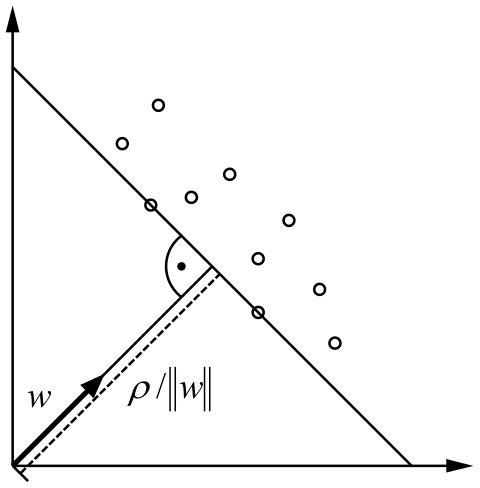
\includegraphics[scale=0.3]{images/svm.png}
    \caption{Lepetit-Ansatz im Diskreten.}
    \label{fig:svm}
\end{figure}

\begin{itemize}
    \item Gaußsche Mischmodelle (GMM):
        \begin{itemize}
            \item Neuheitserkennung (Daten, die nicht trainiert wurden) über Rückweisung mit $k$-sigma-Wahrcheinlichkeit: $$P_{k\sigma}(\boldsymbol{x}) = \frac{\displaystyle\max_{i=1,\dots,m} P(\omega_i) P(k)}{\displaystyle\max_{i=1,\dots,m} P(\omega_i)}$$
            \item Wahrscheinlichkeit, dass ein Merkmalsvektor außerhalb eines $k$-sigma-Ellipsoids um den Mittelwert liegt ($t$ als unterer Schwellwert für die Rückweisung: $P_{k\sigma} \ge t$)
        \end{itemize}
    \item Multilayer Perceptron (MLP):
        \begin{itemize}
            \item Aufgrund der Form der Aktivierungsfunktionen sind Perzeptrons nicht zur Neuheitserkennung geeignet (Softmax-Funktion führt dazu, dass die Aktivierungen in einem Sektor des Merkmalsraums (bis unendlich) den Wert 1 haben)
            \item Für Neuheitserkennung Einführung einer separaten Klasse für Merkmalsvektoren, die zu keiner trainierten Klasse gehören
            \item Für diese Rückweisungsklasse können während des Trainings automatisch Trainingsdaten erzeugt werden:
                \begin{itemize}
                    \item Berechnung des kleinsten umschließenden Hyperquaders der jeweiligen Klasse
                    \item Berechnung  eriner Quaderschale einer gewissen Dicke und eines gewissen Abstandes zum kleinsten umschließenden Hyperquaders jeder Klasse
                    \item Erzeugung von Merkmalsvektoren innerhalb der Quaderschale in den Bereichen, die sich nicht mit den Hyperquadern der anderen Klassen überlappen
                \end{itemize}
            \item Die Neuheitserkennung für CNNs ist ein derzeit noch ungelöstes Problem
        \end{itemize}
    \item Support Vector Machine (SVM):
        \begin{itemize}
            \item Zur Neuheitserkennung Modifikation der SVM
            \item Transformation der Merkmale in den höherdimensionalen Raum
            \item Bestimmung einer Hyperebene (Figure~\ref{fig:svm}) im höherdimensionalen Raum, die maximalen Abstand vom Ursprung besitzt und den Ursprung von den Trainingsdaten $x_i$ trennt
            \item Parametrisiereung der Hyperebene über $(\boldsymbol{w}, \rho)$
            \item Beachte: Es gibt keine Klassenlabel $y_i$
            \item Entscheidungsfunktion: $$f(\boldsymbol{x}) = \sgn \bigg(\sum_{i=1}^l \alpha_i k(\boldsymbol{x}_i, \boldsymbol{x}) - \rho \bigg)$$
            \item $f(\boldsymbol{x}) = -1 \Rightarrow \boldsymbol{x}$ ist neu
            \item Mit den Gaußschen radialen Basisfunktion kann man jeden Trainingsdatensatz vom Ursprung trennen
            \item Um eventuelle Fehler (Ausreißer) in den Trainingsdaten handhaben zu können, wird auch hier ein Parameter $\nu$ eingeführt:
                \begin{itemize}
                    \item $\nu$ ist eine obere Schranke für den Anteil der Ausreißer in den Trainingsdaten
                    \item $\nu$ ist eine untere Schranke für den Anteil der Stützvektoren unter den Trainingsdaten
                \end{itemize}
        \end{itemize}
\end{itemize}


\subsection{Wichtiges Kriterium für die Klassifikation: Ausreichend viele Trainingsdaten}

\begin{itemize}
    \item Wenn eine große Menge an Trainingsdaten verwendet wird, zeichnet sich keines der Verfahren bei gleichen Eingabedaten gegenüber den anderen Verfahren duch eine signifikant höhere Erkennungsrate (niedrigere Fehlerwahrscheinlichkeit) aus
    \item In jedem Fall ist eine große Menge an Trainingsdaten die Voraussetzung für eine hohe Erkennungsrate
\end{itemize}

\section{Beschriftungserkennung}
    \begin{itemize}
        \item \textbf{O}ptical \textbf{C}haracter \textbf{R}ecognition
            \begin{enumerate}
                \item Segmentierung der Zeichen
                \item Klassifikation der Zeichen ("Lesen der Zeichen")
            \end{enumerate}
        $\Rightarrow$ OCR ist die Klassifikation der segmentierten Zeichen
    \end{itemize}
\subsection{Segmentierungsverfahren bei der OCR zur Auftrennung von verschmolzenen Zeichen}
    \begin{itemize}
        \item Schwellwertoperationen: global, dynamisch, automatisch
        \item Beleuchtungskorrektur
        \item Regionen-, Grauwertmorphologie
        \item Alles was situationsspezifisch hilft...
    \end{itemize}
    \begin{itemize}
        \item Industrielle Zeichensätze haben oft konstante Breite $\rightarrow$ Segmentierung in Quadrate gleicher Breite (konstante Auftrennung)
        \item Alternativ: Vorgabe der ungefähren Breite und der möglichen Breitenänderung $\rightarrow$ Suchbereich für Trennlinie $\rightarrow$ Trennlinie an vertikaler Linie mit den geringsten Punkten und minimalem Abstand zur erwarteten Breite (dynamische Auftrennung)
    \end{itemize}

\subsection{Klassifikation bei der OCR basiert auf Regionen- und Grauwertmerkmalen}
    \begin{itemize}
        \item Merkmale:
            \begin{itemize}
                \item Anisometrie
                \item Verhältnis Breite/Höhe des umschließenden Rechtecks
                \item  Anzahl Löcher
                \item Robust kontrastnormierte Grauwerte innerhalb des umschließenden Rechtecks skaliert auf Standardgröße
            \end{itemize}
        \item Probleme
            \begin{itemize}
                \item Ähnlich Zeichen: Cc ,. :;
                \item In der Industrie meist vermieden durch spezielle Zeichensätze
            \end{itemize}
    \end{itemize}

\section{Farbbildverarbeitung}

\subsection{Farbe: Lichtquelle $\rightarrow$ Reflexion, Transmission (Objekt) $\rightarrow$
Wahrnehmung (Auge) $\rightarrow$ Interpretation (Gehirn)}
    \begin{itemize}
        \item sichtbares Lichtspektrum: 380 nm – 780 nm
        \item  Röntgen- und Gammastrahlung $<$ Ultraviolettstrahlung $<$ Sichtbares Licht $<$ Infrarotstrahlung $<$ Mikro- und Radiowellen
        \item Farbspektrum wird am Monitor oder im Druck nicht korrekt widergegeben
        \item Weißes Licht besteht aus allen sichtbaren Wellenlängen, einzelne Wellenlängen dargestellt als spektrale Leistungsdichte
        \item Objekte interagieren mit Licht:
        \begin{itemize}
            \item Transmission (Fensterglas)
            \item Absorption (Schwarz)
            \item Streuung (Milchglas)
            \item Fluoreszenz (umwandeln in andere Wellenlänge: Remission als Fluoreszenz (schnelle Emission) oder Phosphoreszenz (verzögerte Emission))
        \end{itemize}
        \item (ideale) Schwarze Körper absorbieren komplett und geben nur eine zur Wärme proportionales Leistungsspektrum ab
        \item CIE hat feste Spektren für Lichtquellen definiert, Normallichtarten typ D liegen nah am Spektrum Schwarzer Körper
        \item Menschliche Wahrnehmung
        \begin{itemize}
            \item Stäbchen (rods) $\rightarrow$ Nachtsehen (skotopisches Sehen, Hell-Dunkel) $\approx$ 92 Millionen
            \item Zapfen (cones) $\rightarrow$ Tagessehen (photopisches Sehen, Farbwahrnehmung) $\approx$ 4.6 Millionen
            \item 'bunte Tannenzapfen seh ich nur am Tag'
            \item Stäbchen sind $\approx$ Faktor 100 Lichtsensitiver (Dunkelsicht)
            \item L-Zäpfchen maximal effektiv im Rotbereich 566nm (häufigste)
            \item M-Zäpfchen maximal effektiv im Grünbereich, 543nm
            \item S-Zäpfchen maximal effektiv im Blaubereich 440nm (seltenste)
            \item \textbf{Metamerie}
            \begin{itemize}
                \item $\text{Eigenschaft spektral unterschiedlicher Farbreize, die gleiche Farbempfindung auszulösen}_\text{Wikipedia}$
                \item (um Farbreitze zu erzeugen reicht es dem Auge Kompositionen aus R G B zu übermitteln)
                \item Rot, Grün und  Blau (Monitore)
                \item Cyan, Magenta, Gelb (Drucker)
                \item Farbe eines Objekts kann je nach Beleuchtung variieren
            \end{itemize}
            \item Übertragung ans Gehirn via Helligkeitskanal
            \item via Gegenfarbkanäle Rot(+)-Grün(-)-Kanal, Gelb(+)-Blau(-)-Kanal
        \end{itemize}
    \end{itemize}
\subsection{Farbe läßt sich durch drei Farbwerte in einem Farbenraum darstellen}
\begin{itemize}
    \item \textbf{Beschreibungen basierend auf Farbmischung}
    \begin{itemize}
        \item \textbf{rgb}
        \begin{itemize}
            \item Industriestandard bei Digitalkameras, zur direkten Wiedergabe Kalibirierung der Primärfarben des Bildschirms notwendig
            \item kann eine Gammakorrektur enthalten
            \begin{itemize}
                \item $v_{video}^{\gamma} = v_{scene}$
                \item bzw.: $v_{video} = v_{scene}^{1/\gamma}$
                \item NTSC: $\gamma = 2.2$
                \item PAL:   $\gamma = 2.8$
            \end{itemize}
            \item additive Farbmischung
                \begin{itemize}
                    \item (Red , Green, Blue) additive Farbmischung
                    \item (0, 0, 0) = Schwarz
                \end{itemize}
            \item subtraktive Farbmischung
                \begin{itemize}
                    \item (Cyan , Magenta, Gelb) subtraktive Farbmischung
                    \item (0 , 0, 0) = Weiß
                \end{itemize}
            \item Farbraum ist ein Würfel
            \item RGB-Farbenraumdarstellung ist geräteabhängig
            \item Farbgamut (Darstellbarer Bereich) im Auge übersteigt den technischer Geräte
            
        \end{itemize}

    \end{itemize}
    \item \textbf{Beschreibungen basierend auf Farbordnung}
    \begin{itemize}
        \item Signal aufgeteilt in:
        \begin{itemize}
            \item Kanal für Helligkeit (Farbwürfel zu Quader verzogen, so das Leuchtdichte = z-Position)
            \item Farbkanäle (x-, z-Position innerhalb des Farb-Quaders)
        \end{itemize}
        \item \textbf{YIQ}
        \begin{itemize}
            \item NTSC-Farbvideonorm
            \item Y = Leuchtdichte (luminance)([0-Positiv])
            \item I,Q = Farbigkeit (chrominance)([Negativ/Positiv])
        \end{itemize}
        \item \textbf{YUV}
        \begin{itemize}
            \item Y = Leuchtdichte(luminance)([0-Positiv])
            \item U, V =  Farbigkeit (chrominance)([Negativ/Positiv])
        \end{itemize}
    \end{itemize}
    \item \textbf{Farbenräume basierend auf Farbordnung}
        \item Intuitive Beschreibung der Farbe
        \begin{itemize}
            \item basierend auf Helligkeit (lightness), Buntton (hue) und  Sättigung (saturation) oder Buntheit (chroma)
            \item Vorteile
            \begin{itemize}
                \item Buntton und Sättigung (in HLS) sind semantisch sinnvolle Attribute
            \end{itemize}
            \item Nachteile
            \begin{itemize}
                \item Helligkeit ist kein semantisch sinnvolles Attribut(reines Blau gefühlt dunkler als reines Grün)
                \item Darstellung ist Geräteabhängig
                \item Farbunterschide sind gefühlt nicht gleichförmig
            \end{itemize}
            \item \textbf{HSI}
            \begin{itemize}
                \item Intensität I = Diagonale des RGB-Farbraums (alle unbunten Farben)
                \item Polarkoordinatensystem orthogonal zur Intensität
                \begin{itemize}
                    \item Winkel = Buntton (Konvention $0^\circ$ = Rot) (durch Quaderform nicht einheitlich)
                    \item Abstand = Sättingung (durch Quaderform nicht einheitlich)
                    \item eine direkte Umrechnung aus RGB-Raum $\rightarrow$ Farbenraumdarstellung Geräteabhängig
                \end{itemize}
            \end{itemize}
            \item \textbf{HLS}
            \begin{itemize}
                \item umgerechnet aus HSI 
                \item Buntton (Hue) ist einheitlich, Diamantform
                \item Helligkeit (Lightness)
                \item Sättigung (Saturation) (echte Sättigung, Buntheit/Helligkeit  ist einheitlich)
                \item Standard in Grafikprogrammen
            \end{itemize}
            \item \textbf{HSV}
            \begin{itemize}
                \item Buntton (Hue) (reine Farbe hat Helligkeit 1)
                \item Sättigung (Saturation)
                \item Value (Buntheit (Kegel) oder Sättigung (Zylinder))
            \end{itemize}
        \end{itemize}
    \item \textbf{Beschreibungen basierend auf Farbabgleich}
    \begin{itemize}
        \item Farbabgleich (color matching) = experimentelles Mischen von 3 Primärvalenzen (Farbiges Licht) um gegebene Farbe zu erzeugen
        \item bestimmte Testfarben nicht durch die drei Primärvalenzen dargestellt werden
        \item  Primärvalenzen mit Menschen Ergaben Farbenräume
        \item 'Farbleistung' skaliert und addition und subtraktion von Farben ist möglich)
        \item CIE definiert Farbraum für Normalbeobachter mit $2^\circ$ Sichtfeld und $10^\circ$ ohne innere $2^\circ$ Sichtfeld
        \item repräsentieren die durchschnittliche menschliche Farbwahrnehmung
        \item Die Farbwahrnehmung einer echten Person kann sich erheblich vom Normalbeobachter unterscheiden (Biologisch \& Altersbedinkt)
    \end{itemize}
        \item \textbf{CIE-XYZ-Farbwerte}
        \begin{itemize}
            \item es gilt X, Y, Z (Farbvalenzen) werden normiert zu x, y, z (Farbwertanteile)
            \item es gilt: x + y + z = 1, daher reichen (x, y) + Y zur rücktransformation
            \item (x,y) ergibt eine Hufeisenförmige Visualisierung der Menschen wahrnehmbaren Farbarten
            \item wird oft zur beschreibung der Primärfarben von Ausgabegeräten genutzt
            \item sind Primärfarben des Ausgabegerätes als CIE-XYZ-Farbvalenzen bekannt, kann der jeweilige RGB Wert errechnet werden
            \item erlaubt den Vergleich zweier Farbdarstellungen auf unterschiedlichen Geräten
            \item Farbraum ist nicht gleichförmig, Regionen unterschiedlicher Größe können für Menschen einfarbig aussehen, gerade im oberen Bereich
        \end{itemize}
    \item \textbf{CIELUV}
    \begin{itemize}
        \item Farbraum ist näherungsweise gelichförmig (durch projektive Transformation auf wahrgenommene Veränderung angepasst)
        \item ergibt UCS (uniform chromaticity scale) diagram
        \item ist auf CIE-Normlichtart D65 ausgelegt, so das es nur in Kontrollierter Beleuchtung eingesetzt werden sollte
        
    \end{itemize}
    \item \textbf{$\text{CIELCh}_\text{uv}$}
        \begin{itemize}
            \item CIELUV in Polarkoordinaten
        \end{itemize}
    \item \textbf{CIELAB}
    \begin{itemize}
        \item wie CIELUV mit anderer projektiver Transformation
    \end{itemize}
    \item \textbf{$\text{CIELCh}_\text{ab}$}
    \begin{itemize}
        \item  CIELAB in Polarkoordinaten
    \end{itemize}
    
\end{itemize}

\subsection{Prinzip des Farbmanagements}

\begin{itemize}
    \item Falls eine Transformation der RGB-Rarbwerte der Kamera in CIE-XYZ-Farbwerte (mit möglichst kleinem Fehler) bestimmt worden ist, ist die Kamera farbkalibriert ($\Rightarrow$ Kamera unterliegt somit einem Farbmanagement)
    \item Das Farbmanagement dient dazu, die menschliche Wahrnehmung möglichst gut nachzubilden
    \item Je nach spektralem Empfindlichkeitsgrad der Kamerasensoren können bestimmte Farben mehr oder weniger korrekt beschrieben werden
    \item Die unterschiedliche Bahandlung von Metamerie bei Mensch und Kamera kann durch Farbmanagement nicht nachträglich korrigiert werden
    \item Zur Bestimmung der Transformation von RGB zu CIE-XYZ wird eine Farbkalibriertafel (besitzt eine bestimmte Anzahl von Feldern, für die die CIE-XYZ-Farbwerte (oder CIE-Yxy-Farbwerte) bekannt sind) verwendet
    \item Vorab muss radiometrische Kalibrierung der Kamera durchgeführt werden, um eventuelle Nichtlinearitäten der RGB-Farbwerte zu entfernen
    \item Die Farbkalibrierung erfolgt durch Minimierung der Fehler der transformierten linearen RGB-Farbwerte und der XYZ-Farbwerte der Rarbkalibriertafel
    \item Transformation oft als linear angenommen, ansonsten quadratische Transformation
\end{itemize}

\subsection{Prinzip der chromatischen Adaption}
\begin{itemize}
    \item kalibrierte Farbwerte sind nur für die Beleuchtung gültig in der sie kalibriert wurden
        \item Veränderung des Spektrums abhängig von
        \begin{itemize}
            \item Tageszeit, Standort, Bewölkung
        \end{itemize}
        \item Auswirkung:
        \begin{itemize}
            \item Farbwerte ändern sich
            \item für Menschen erscheinen unbunte Farben schnell bunt
        \end{itemize}
        \item für hohe Genauigkeit muss eine erneute Kalibrierung durchgeführt werden
        \item für geringe Genauigkeit reicht eine chromatic adaptation transformation (CAT)
        \begin{itemize}
            \item Hauptziel ist die Wiederherstellung der Unbuntheit der unbunten Farben, daher der Beiname \textbf{Weißabgleich}
            \item Annahme: Unbunte Farben führen zu identischen Aktivierungen der Zapfen $(L_a = M_a = S_a)$
            \item Annahme:Empfindlichkeit der Zapfen(Farbsicht) passt sich der Beleuchtung linear an
            \item wird typischerweise auf CIEXYZ Farbraum durchgeführt, kann bei bekannten Transformationsmatrizen aus anderen Farbräumen transformiert werden und durch Inversion der Matrix wieder zurück
            \item nichtlineare Kodierung der Farbwerte muss vorher entfent werden(Gammakorrektur etc.)
            \item Druchführung:
            \begin{itemize}
                \item ggf. inverse Gammakorrektur
                \item Farbwerte aus einem geräteunabhängigen Farbraum transformieren
                \item Vehältniss der Echten und transformierten CIEXYZ-Farbwerte berechnen
                \item Bild transformieren
            \end{itemize}
            \item bei unbekanntem Beleuchtungsspektrum(Normalfall) kann die chromatische Adaption basierend auf einer weißen Region im Bild durchgeführt werden
            \item Automatischer Weißabgleich wie in Kameras kann durch einige Approximationen algorythmisch automatisiert werden:
            \begin{itemize}
                \item Die Welt ist im Mittel grau: die Mittelung aller Farben im Bild ergibt ein Grau mit $18\%$ Helligkeit
                \item Die hellste Farbe im Bild ist weiß
                \item Analyse des Farbgamuts des aufgenommenen Bildes und statistischer Vergleich mit Farbgamutdaten aus einer Datenbank
            \end{itemize}
        \end{itemize}
\end{itemize}

\subsection{Prinzip des Demosaicking}

\begin{itemize}
    \item CCD- und CMOS-Sensoren können verschiedene Farben (also unterschiedliche Wellenlängen) nicht unterscheiden
    \item Um Farbbilder aufzunehmen, existieren zwei verschiedene Technologien:
        \begin{itemize}
            \item Drei-Chip-Kameras
            \begin{itemize}
                \item verwenden ein Prisma als Strahlenteiler, um das einfallende Licht auf drei Sensoren umzulenken
                \item Vorteil: Das Bild hat die volle Auflösung in jeder Farbe
                \item Nachteil: Deutlich höherer Preis
            \end{itemize}
            \item Ein-Chip-Kameras 
            \begin{itemize}
                \item besitzen nur einen Sensor mit derselben Auflösung wie ein Schwarzweiß-Sensor
                \item Hier werden die Filter für die drei Grundfarben in einer Mosaikanordnung vor dem Sensor angebracht
                \item Nachteil: Die Auflösung der Farbkanäle ist unterschiedlich und geringer als die Auflösung eines Schwarzweiß-Sensors
                \\ $\Rightarrow$ Die Farbinformation muss interpoliert werden (sog. Demosaicking)
            \end{itemize}
        \end{itemize}
\end{itemize}

\subsection{Methoden zur Segmentierung von Farb- und Mehrkanalbildern}

\begin{itemize}
    \item 
\end{itemize}

\subsection{Prinzip der Kanten-, Linien- und Punktextraktion über den metrischen Tensor des Farb- oder Mehrkanalbildes}

\begin{itemize}
    \item 
\end{itemize}


\section{Hand-Auge-Kalibrierung}

\subsection{Koordinatensysteme und –transformationen}

\begin{itemize}
    \item beschrieben durch \textbf{Ursprung} und \textbf{$n$ orthogonale Achsen} (Einheitsvektoren)
    \item \textbf{rechts}- und linkshändige
    \item Transformation von einem zum anderen: \textbf{starre Abbildung im n-dimensionalen Raum}
    \item Ursprung von einem KS ist Punkt, der in anderem dargestellt werden kann (Translationsvektor)
    \item Rotationsmatrix: Achsen von einem KS in anderem ausgedrückt: 
    \item $x_1^{\{0\}} = \boldsymbol{R}_1^0 x_1^{\{1\}} \Rightarrow \boldsymbol{R}_1^0 = \begin{bmatrix} x_1^T x_0 && y_1^T x_0 \\ x_1^T y_0 && y_1^T y_0 \end{bmatrix}$ (alle Vektoren in KS $\{0\}$)
    \item $\boldsymbol{R}_0^1 = \begin{bmatrix} x_0^T x_1 && y_0^T x_1 \\ x_0^T y_1 && y_0^T y_1 \end{bmatrix}$ (alle Vektoren in KS $\{0\}$)
    \item $\boldsymbol{R}_0^1 = (\boldsymbol{R}_1^0)^T = (\boldsymbol{R}_1^0)^{-1}$
    \item orthogonale Matrizen: a) $det(\boldsymbol{R}) = 1$ Rotationen, b) $det(\boldsymbol{R}) = -1$ Spiegelungen
    \item $p^{\{0\}} = \begin{bmatrix} p^{\{1\}T} x_0^{\{1\}} && p^{\{1\}T} y_0^{\{1\}} && p^{\{1\}T} z_0^{\{1\}} \end{bmatrix}^T = \boldsymbol{R}_1^0 p^{\{1\}}$
    \item Drehung Objekt von $p_a$ zu $p_b$: $p_b^{\{0\}} = \boldsymbol{R}_1^0 p_b^{\{1\}} = \boldsymbol{R}_1^0 p_a^{\{0\}}$
    \item $\boldsymbol{R}_2^0 = \boldsymbol{R}_1^0 \boldsymbol{R}_2^1$
    \item starre Abbildung: $p^{\{0\}} = \boldsymbol{R}_1^0 p^{\{1\}} + t_1^0 = \boldsymbol{R}_1^0 \boldsymbol{R}_2^1 p^{\{2\}} + \boldsymbol{R}_1^0 t_2^1 + t_1^0 $
    \item homogene Koordinaten: $\boldsymbol{H} = \begin{bmatrix} \boldsymbol{R} && t \\ \boldsymbol{0}^T && 1 \end{bmatrix}$, $p_{hom} = \begin{bmatrix} p \\ 1 \end{bmatrix}$, $\boldsymbol{H}^{-1} = \begin{bmatrix} \boldsymbol{R}^T && - \boldsymbol{R}^T t \\ \boldsymbol{0}^T && 1 \end{bmatrix}$
    \item 2D Rotationen $\boldsymbol{R} = \begin{bmatrix} \cos{\theta} && -\sin{\theta} \\ \sin{\theta} && \cos{\theta} \end{bmatrix}$, $z = x + iy = r(\cos{\theta} + i \sin{\theta}) = r e^{i\theta}$
\end{itemize}


\subsubsection{Eulerwinkel}
\begin{itemize}
    \item Aufsplittung in 3 Rotation um orthogonale Achsen
    \item 12 versch. Sequenzen möglich
    \item $\boldsymbol{R}_x = \begin{bmatrix} 1 && 0 && 0 \\ 0 && \cos{\theta} && - \sin{\theta} \\ 0 && \sin{\theta} && \cos{\theta} \end{bmatrix}$, $\boldsymbol{R}_y = \begin{bmatrix} \cos{\theta} && 0 && \sin{\theta} \\ 0 && 1 && 0 \\ - \sin{\theta} && 0 && \cos{\theta} \end{bmatrix}$, $\boldsymbol{R}_z = \begin{bmatrix} \cos{\theta} && - \sin{\theta} && 0 \\ \sin{\theta} && \cos{\theta} && 0 \\ 0 && 0 && 1 \end{bmatrix}$
\end{itemize}


\subsubsection{Rotationsachse und Rotationswinkel}
\begin{itemize}
    \item Rotationsachse $n$, Rotationswinkel $\theta$, $||n|| = 1$
    \item Rodrigues Formel: $\boldsymbol{R} = I + \sin{\theta} [n]_{\times} + (1 - \cos{\theta}) [n]_{\times}^2$ ($[n]_{\times} = \begin{bmatrix} 0 && -n_3 && n_2 \\ n_3 && 0 && -n_1 \\ -n_2 && n_1 && 0 \end{bmatrix}$)
    \item von Rotationsmatrix zu Rotationsachse: Eigenvektor zum Eigenwert $1$, $\theta$ aus $e^{i\theta}$ oder $e^{-i\theta}$
\end{itemize}

\subsubsection{Quaternionen}
\begin{itemize}
    \item 3fach komplexe Zahlen ($i, j, k$), $\boldsymbol{q} = \begin{bmatrix} q_0 && q_1 && q_2 && q_3 \end{bmatrix}^T = \begin{bmatrix} q_0 && q_v^T \end{bmatrix}^T$
    \item $\boldsymbol{p}\boldsymbol{q} = \begin{bmatrix} p_0 q_0 - p_v^T q_v && (p_0 q_v + q_0 p_v + p_v \times q_v)^T \end{bmatrix}^T$
    \item $\boldsymbol{\bar{q}} = \begin{bmatrix} q_0 && -q_v^T \end{bmatrix}^T$
    \item $\boldsymbol{p}\boldsymbol{q} \neq \boldsymbol{q}\boldsymbol{p}$
    \item $\boldsymbol{q}^{-1} = \frac{\boldsymbol{\bar{q}}}{\boldsymbol{q}\boldsymbol{\bar{q}}}$
    \item von Rotationsvektor zu Quaternion: $\boldsymbol{q} = \begin{bmatrix} \cos{(\frac{1}{2} \theta)} && \sin{(\frac{1}{2} \theta)} n^T \end{bmatrix}^T$
    \item Punkt rotieren: $\boldsymbol{p} = \begin{bmatrix} 0 && p^T \end{bmatrix}^T$, $\boldsymbol{p}_{rot} = \boldsymbol{q}\boldsymbol{p}\boldsymbol{\bar{q}}$
    \item $\boldsymbol{q}$ und $-\boldsymbol{q}$ beschreiben gleiche Rotation
\end{itemize}

\subsubsection{Schraubungen}
\begin{itemize}
    \item Gerade $g = p + \lambda (q-p) = p + \lambda l$
    \item Plückerkoordinaten: $l = q -p $ und $m = p \times l = p \times q$, $l$ normieren
    \item homogene Plückerkoordinaten: $l_{ij} = -l_{ji} = p_i q_j - p_j q_i$, $l = \begin{bmatrix} -l_{14} && l_{42} && -l_{34} \end{bmatrix}^T$ and $m = \begin{bmatrix} l_{23} && -l_{13} && l_{12} \end{bmatrix}^T$
    \item von $\boldsymbol{R}, t$ auf Schraubung: $l, \theta$ = Rotationsachse und -winkel von $\boldsymbol{R}$, $d = t^T l$, $m = \frac{1}{2} (t \times l + (t - dl) \cot{(\frac{1}{2} \theta)})$
    \item von Schraubung zu $\boldsymbol{R}, t$: R - Rodrigues Formel, $t = (I - R) (l \times m) + dl$
    \item Punkt auf g mit kürzesten Abstand zu Ursprung: $l \times m$
\end{itemize}


\subsubsection{Duale Quaternionen}
\begin{itemize}
    \item $\boldsymbol{\hat{q}} = \begin{bmatrix} \hat{q}_0 && \hat{q}_1 && \hat{q}_2 && \hat{q}_3 \end{bmatrix}^T = \begin{bmatrix} \hat{q}_0 && \hat{q}_v^T \end{bmatrix}^T$
    \item $\boldsymbol{\hat{p}}\boldsymbol{\hat{q}} = \begin{bmatrix} \hat{p}_0 \hat{q}_0 - \hat{p}_v^T \hat{q}_v && (\hat{p}_0 \hat{q}_v + \hat{q}_0 \hat{p}_v + \hat{p}_v \times \hat{q}_v)^T \end{bmatrix}^T$
    \item $\boldsymbol{\bar{\hat{q}}} = \begin{bmatrix} \hat{q}_0 && -\hat{q}_v^T \end{bmatrix}^T$
    \item Geraden in Plückerkoordinaten durch duale Einheitsquaternionen: $\hat{l} = \begin{bmatrix} 0 && \hat{l}_v^T \end{bmatrix}^T = \begin{bmatrix} 0 && l^T \end{bmatrix}^T + \epsilon \begin{bmatrix} 0 && m^T \end{bmatrix}^T$
    \item von Schraubung zu duales Einheitsquaternion: $\hat{q} = \begin{bmatrix} \cos{(\frac{1}{2}\hat{\theta})} && \hat{n}^T \sin{(\frac{1}{2} \hat{\theta})} \end{bmatrix}^T$, $\hat{n} = n + \epsilon o$, $||n|| = 1$, $n^T o=0$, $\hat{\theta} = \theta + \epsilon d$
\end{itemize}

\subsection{Koordinatensysteme an Robotern}

\begin{figure}[h!]
    \begin{subfigure}[c]{0.5\textwidth}
        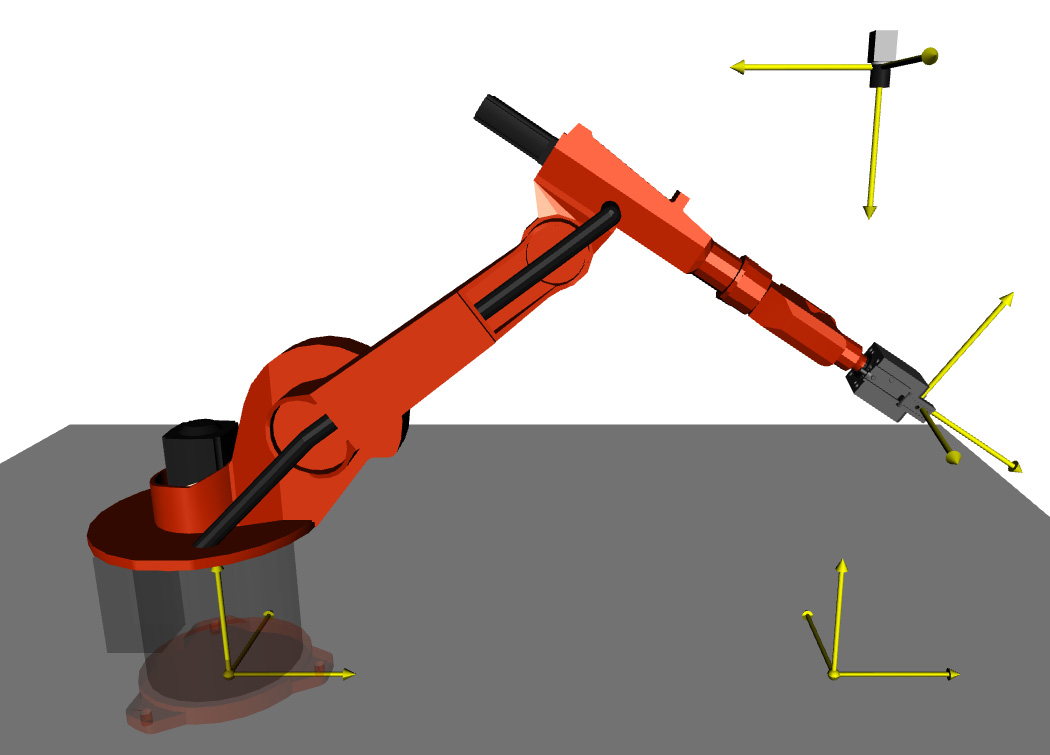
\includegraphics[width=\linewidth]{images/stationaere_kamera.png}
        \subcaption{stationäre Kamera}
    \end{subfigure}%
    \begin{subfigure}[c]{0.5\textwidth}
        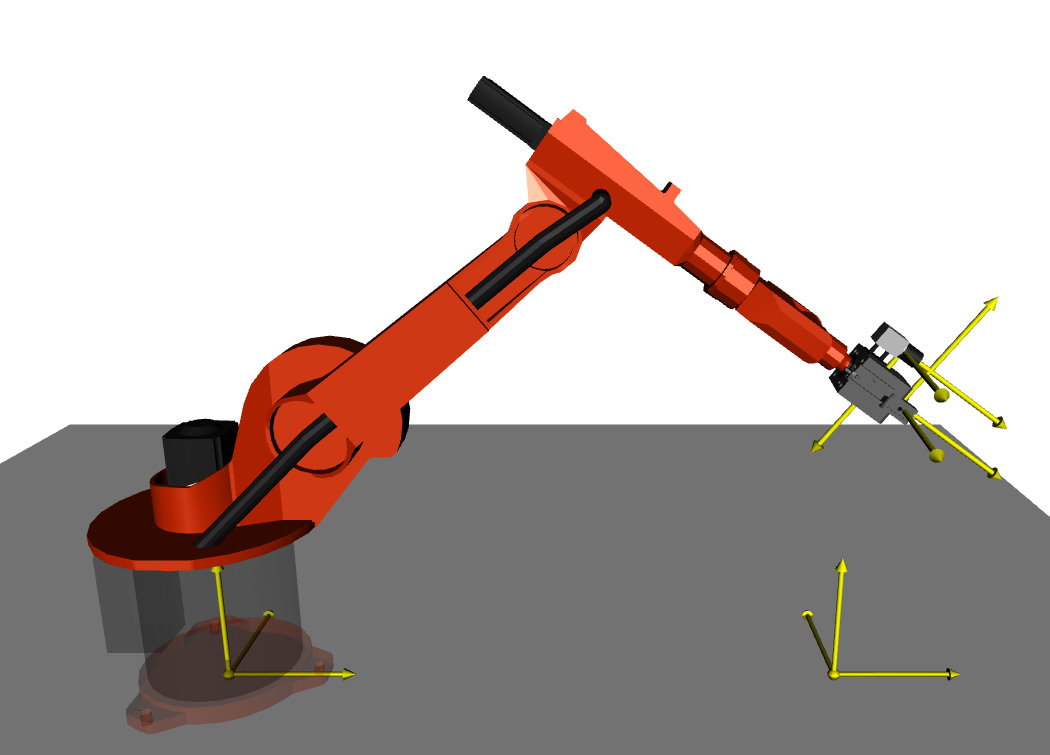
\includegraphics[width=\linewidth]{images/bewegte_kamera.png}
        \subcaption{bewegte Kamera}
    \end{subfigure}
\end{figure}

\subsection{Problemdefinition (stationäre und bewegte Kamera)}

\subsubsection{stationäre Kamera}
\begin{itemize}
    \item außerhalb Roboter
    \item beobachtet Arbeitsraum von Roboter
    \item Problem: bestimme Lage Kamerakoordinatesnsystem relativ zu Basiskoordinatensystem
    \item Kalibrierkörper wird in $n$ unterschiedlichen Posen bewegt
    \item gesucht: Basis $\rightarrow$ Kamera, Tool $\rightarrow$ Endeffektor
\end{itemize}

\subsubsection{bewegte Kamera = Auge-in-Hand-Konfiguration}
\begin{itemize}
    \item am Endeffektor montiert
    \item Problem: bestimme Lage Kamerakoordinatesnsystem relativ zu Werkzeugkoordinatensystem
    \item Kamera wird in $n$ unterschiedliche Posen bewegt
    \item gesucht: Kamera $\rightarrow$ Endeffektor, Kalibrierkörper $\rightarrow$ Basis
\end{itemize}


\subsection{Lösungsmethoden}

\subsubsection{Ansätze, die Gleichungen der Form $AX = XB$lösen}

\subsubsection{Ansätze, die Gleichungen der Form $AX = YB$lösen}

\subsubsection{Optimale Hand-Auge-Kalibrierung}


\section{Objekterkennung}

\subsection{Prinzip des deskriptorbasierten Matchings}

\begin{itemize}
    \item Homographie (projektive Transformation) $H$: $p_i' = \lambda_i Hp_i$ ($\lambda$ - unbekannter Skalierungsfaktor) $\Rightarrow p_i' \times Hp_i = 0$
    \item direct linear transformation (DLT)
    \item mindestens 4 Punkte benötigt, numerisch instabil (leichte Verbesserung durch Normalisierung)
    \item besser: bundle adjustment (Bündelausgleich), mehr Rechenaufwand
    \item Punkt-Gerade-Korrespondenz: $l^T H^{-1} p' = 0$ $\rightarrow$ analog zu Punkten, aber min. 8 Korrespondenzen
    \item Weltkoordinaten schätzen: bekannt: interne Kameraparameter + Sehstrahlen durch Merkmale, zusätzlich benötigt: Entfernung Modellebene oder Kalibrierkörper
    \item Kameramatrix $K = \begin{bmatrix} \frac{f}{s_x} && 0 && c_x \\ 0 && \frac{f}{s_y} && c_y \\ 0 && 0 && 1 \end{bmatrix}$, Kamerapose $P = \begin{bmatrix} R && t \end{bmatrix}$, $R = K^{-1}H$
    \item Modellpose berechnen: Distanzen zwischen projizierten Geraden und korrespondierten Kantenpunkten minimieren
    \item langes Training, schnelle Suche
    \item benötigt viel Textur
    \item keine repetetive Texturen
\end{itemize}

\subsubsection{Extraktion von markanten Punkten}
\begin{itemize}
    \item im Modell und Suchbild markante Punkte extrahieren, wiederfinden mit Deskriptoren
    \item stabil unter Lageänderung, Skalierung, Rotation, Beleuchtung
    \item Punktextraktion mittels Harris, Lepetit
\end{itemize}

\subsubsection{Klassifikation der Punkte im Suchbild}
\begin{itemize}
    \item Korrespondenzsuche ist Klassifikationsproblem (jeder Modellpunkt eigene Klasse), Lösung: randomisierte Bäume
    \item zum Training Daten generieren (skalieren, kippen, rotieren)
    \item randomized Trees: an jedem Knoten werden 2 zufällige Punkte aus der Umgebung verglichen
\end{itemize}

\subsubsection{Hypothesengenerierung und –validierung über RANSAC}
\begin{itemize}
    \item wähle $s$ (genug um Modellparameter zu schätzen) zufällige Datenpunkte aus -> Modelparameter
    \item Konsensmenge berechnen (Punkte die max. Abstand $d$ zu Modell haben)
    \item wiederholen
    \item Modellparameter mit größter Konsensmenge verwenden
\end{itemize}

\subsection{Prinzip des deformierbaren Matchings}
\begin{itemize}
    \item zerlege Objekt in mehrere Teile (Clustering)
    \item Erzeuge Hypothesen auf oberster Pyramidenstufe durch template matching
    \item Match durch Pyramide tracken, Hypothese verfeinern
    \item auf unterster Stufe Homographie, Pose oder Deformation bestimmen
    \item auch als Tracking verwendbar
    \item Deformation durch Vektorfeld (über Punktkorrespondenzen)
    \item gut für Ojekte mit Kanten
    \item Training schnell
    \item Suche relativ schnell
    \item nicht geeignet für kleine Objekte oder dünne Linien (verschwinden aus Bildpyramide)
\end{itemize}

\subsection{Prinzip des ansichtenbasierten Matchings}
\begin{itemize}
    \item für Objekte mit wenig Textur, aber Kanten
    \item 3D-CAD Modell verfügbar
    \item virtuelle Kameras auf Schale um Objekt platzieren
    \item Kanten mit renderings matchen - Pose von Rendering verwenden mit 2D Matching-Parameter verfeinern
    \item sehr rechenaufwendig, geringe Genauigkeit, nur orthographische Projektion (Objekt in Mitte)
\end{itemize}

\subsection{Prinzip des kantenbasierten 3D-Matchings}
\begin{itemize}
    \item wie ansichtenbasiert
    \item Suchraumeinschränkung
    \item erst Überabtastung (Kanten im virtuellen benachbarten Bildern liegen max. 1 Pixel auseinander)
    \item Ausdünnen benachbarter Ansichten, falls Ähnlichkeit bei Templatematching groß, Verwendung Bildpyramiden
    \item Representation in Baumstruktur
    \item robustes Templatematching entlang Baumstruktur
    \item robuster: 3-Kanal Bild: Modellflächen erhalten Grauwerte je nach Normalenvektor
    \item Tracking geeignet
\end{itemize}

\subsection{3D Aufnahme}
\begin{itemize}
    \item Stereo-Setup
    \item Flächenlaser
    \item strukturiertes Licht (Kinect)
    \item Radar, Lidar, Time-of-Flight
    \item Iterative-Closest-Point-Algorithmus: Lage 2er Punktwolken abgleichen aufgrund von Korrespondenzen und Abstandsminimierung
    \item Korrespondenzfindung über k-d-Bäume, Voxel, vollständige Suche
    \item 3D Deskriptoren: Spin-Images, Punktpaarhistogramme
\end{itemize}

\subsection{Prinzip des oberflächenbasierten 3D-Matchings}
\begin{itemize}
    \item Datenbank von Punktpaaren: Abstand, Winkel zw. Normalen, Winkel zw. Normalen und Differenzvektor
    \item diskretisierter Merkmalsvektor als Hashschlüssel
    \item pro: finden in konstanter Zeit, invariant gegenüber starren Abbildungen, 2 Korrespondenzen reichen aus
    \item Größe ist quadratisch zur Zahl der abgetasteten Punkte
    \item für jeden Referenzpunkt in Szene Hough-Transformation
    \item Referenzpunkt mit allen anderen Punkten als Paar in DB gesucht
    \item jeder Referenzpunkt gibt Lagehypothese: Non-Maximum-Suppression
    \item Verfeinerung mit ICP
\end{itemize}

\end{document}
